\chapter{Обоснование эффективности применения разрабатываемой подсистемы}

Разрабатываемую подсистему, из-за своей специфики, можно отнести к классу
открытых систем. Одним из важных признаков таких систем является повышенная безопасность.
~\cite{zapechnikov}

Дадим определения основных понятий, которыми в дальнейшем будем пользоваться при
рассмотрении вопросов защиты.

Под термином \textit{<<информационная безопасность>>}, согласно определению
Гостех-комиссии при Президенте РФ, понимают состояние защищенности информации,
обрабатываемой средствами вычислительной техники или автоматизированной системы,
от внутренних или внешних угроз:
от нежелательного ее разглашения (нарушения конфиденциальности), искажения
(нарушения целостности), утраты или снижения степени доступности информации, а
также ее незаконного тиражирования, которые приводят к материальному или
моральному ущербу владельца или пользователя информации.~\cite{ruk_doc}

\textit{Угрозы (threats)} --- потенциально возможное событие, действие или
процесс, которые посредством воздействия на компоненты системы могут привести к
нанесению ущерба. Это также и люди или группы людей, способные взломать
компьютерную систему.~\cite{gerasimenko} Это может быть любопытный подросток,
рассерженный служащий или шпион конкурирующей компании или иностранного правительства.
Наличие угрозы необязательно означает, что она реализуется и нанесет вред.

\textit{Уязвимость (vulnerability)} --- любая характеристика или свойство
системы, использование которой нарушителем может привести к реализации угрозы. Иными
словами, это слабые места в системах~\cite{gerasimenko}. Уязвимости могут использоваться для
компрометации (взлома) систем.

\textit{Вторжение (intrusion)} --- процесс попытки несанкционированного
проникновения в какую-либо систему. Под вторжением может пониматься любое действие нарушителя,
приводящее к реализации угрозы путем использования уязвимостей. Поэтому это
реализовавшаяся угроза.

\textit{Атака (attack)} --- это событие (момент), при котором злоумышленник
проникает внутрь системы или совершает по отношению к ней какое-либо несанкционированное
действие. Атака является результатом вторжения.

Все нарушители могут быть разделены на две категории:
\begin{enumerate}
  \item Аутсайдеры (outsiders) --- это внешние нарушители по отношению к
  открытой сети, которые атакуют внутренние сетевые ресурсы (цель -- удаление
  информации на корпоративном веб-сqервере, пересылка спэма через почтовый сервер и т.д.). 
  Злоумышленники могут осуществлять атаки из Интернета через модемные линии, через физическое 
  подключение к каналам связи или из сети партнеров (поставщиков, заказчиков, дилеров и т.д.).
  \item Инсайдеры (insiders) --- это внутренние нарушители, находящиеся внутри
  сети и имеющие полный доступ ко всем ее серверам. Это пользователи,
  неправильно применяющие свои привилегии или исполняющие роль
  привилегированного пользователя (например, с привилегированного терминала).
  Исследования показывают, что 80 \% всех атак в сетях исходит именно от
  инсайдеров. Заметим, что существующие методы безопасности не обеспечивают
  защиту от них. Внутренние злоумышленники представляют основную опасность, так
  как они знакомы с системой зашиты, направлением деятельности компании и могут
  реально оценить стоимость ресурсов корпоративной сети. В этой категории опасность 
  представляют уволенные и обиженные сотрудники, мстящие от обиды, <<продвинутые>> 
  пользователи, при каждом удобном случае желающие продемонстрировать свои
  знания, и администраторы, которые в силу своих обязанностей знают многие секреты организации.
\end{enumerate} 

Внутренние злоумышленники по характеру действий могут быть разделены на
следующие категории:
\begin{itemize}
  \item Посторонние лица (у которых права в действующей ИС отсутствуют) осуществляют
перехват или воздействие на информацию, передаваемую по телекоммуникационным
сетям, а также квалифицированное воздействие на систему защиты и работу ИС в
целом с использованием телекоммуникационных сетей.
  \item Разработчики приложений (у которых права в действующей ИС отсутствуют) к уже
названным двум действиям добавляют на этапе разработки ПО реализацию
преднамеренных скрытых возможностей для последующего входа в систему или
непреднамеренных ошибок.
  \item Обслуживающий персонал (у которого права в ИС и на уровне приложений
отсутствуют, но имеется доступ к техническим средствам и ПО) может вести себя
как постронее лицо, плюс получать доступ к сетевому и телекоммуникационному
оборудованию, устанавливать посторонние программы и внедрять программные
закладки.
  \item Пользователи ИС --- сотрудники или клиенты (права на доступ к приложениям ИС)
-- осуществляют перехват или воздействие на информацию, передаваемую по
телекоммуникационным сетям, вносят вредоносное ПО в ИС и присваивают полномочия
других пользователей (в том числе администратора).

В основном их цели сводятся к следующему:
\begin{itemize}
  \item финансовой выгоде;
  \item политической выгоде -- небольшой, но существенный, процент атакующих
  делают это по политическим соображениям, например, они пытаются таким образом
  обратить внимание общественности на отдельную проблему (права животных,
  контроль за оружием, свобода слова и т.д.);
  \item разрушению;
  \item мести недовольных сотрудников;
  \item вызову обществу;
  \item самоутверждению (например, дети хотят поразить друзей своими знаниями и
  навыками);
  \item спорту -- возможно, администратор хвастается защищенностью своего
  интранета, говоря всем, что он непроницаем; перед таким вызовом нарушитель устоять не может;
  \item шутке.
\end{itemize}
\end{itemize}

Угрозы осуществляются на практике в результате стечения случайных обстоятельств
(ошибки, пропуски, сбои электроэнергии, природные бедствия) либо из-за
преднамеренных действий злоумышленников. Общепринятой классификации угроз
безопасности пока не существует.

Возможна классификация угроз безопасности по следующим признакам:
\begin{enumerate}
  \item Цели реализации (цели могут быть связаны, например, со свойствами
  конфиденциальности, целостности и доступности информации, которые собирается
  нарушить злоумышленник, или с расширением прав доступа и получением полного
  контроля над работой компьютера пользователя или определенным сервером);
  \item принципу воздействия на систему (например, взлом парольной защиты или
  нападение на основе сетевого протокола);
  \item характеру воздействия на систему (например, пассивный перехват трафика
  или активная подмена данных);
  \item причине появления используемой ошибки защиты (например, из-за отсутствия
  средств обнаружения вторжений, неправильной настройки средств защиты или не
  установки защищающих обновлений);
  \item объекту атаки (например, данные, программы, сетевое обеспечение);
  \item используемым средствам атаки;
  \item состоянию объекта атаки (например, явное изменение состояния или
  отсутствие каких бы то ни было изменений, так как осуществляется лишь
  пассивный перехват входящих и исходящих пакетов или почтовых сообщений);
  \item по источнику угроз и т. п.
\end{enumerate}

Согласно ставшему уже классическим подходу для информации вообще выделяются три
вида угроз, связанные с ее основными свойствами:
\begin{enumerate}
  \item Угрозы конфиденциальности (конфиденциальность --- защищенность
  информации от несанкционированного ознакомления с нею, подразумевающая
  некоторую классификацию данных, получение либо использование которых
  неавторизованными для этого лицами может стать причиной серьезного ущерба для
  владельцев или пользователей этой информации); примеры угроз: хищение
  (копирование) информации и средств ее обработки, утрата (неумышленная потеря,
  утечка) информации и средств ее обработки.
  \item Угрозы целостности (целостность --- состояние, при котором данные,
  представленные в компьютере, в точности соответствуют данным в исходных
  документах и при этом не могут быть подвержены неумышленным или умышленным
  искажениям или разрушениям; информация может пострадать от сознательных
  действий злоумышленника, от ошибок персонала, от пожара, аварий и др.);
  примеры угроз: модификация (искажение) информации, отрицание ее подлинности,
  навязывание ложной информации.
  \item Угрозы доступности (доступность --- возможность за приемлемое время
  получить требуемую информационную услугу, причем наличие системы безопасности
  не должно создавать помех нормальной работе системы); примеры угроз:
  блокирование информации; уничтожение информации и средств ее обработки.
\end{enumerate}
 
Анализ всего комплекса угроз и оценка последствий их реализации составляет одну
из первых задач сотрудников, ответственных за безопасность. Оценка уязвимости
систем предполагает изучение всех комбинаций реализации перечисленных угроз и
последствий, к которым они приводят. По мере совершенствования средств и методов
защиты компьютерных систем злоумышленниками создаются новые, весьма изощренные
способы их преодоления. Приведем здесь перечень наиболее вероятных случайных
происшествий и злоумышленных действий, которые важны при оценке степени
уязвимости любой системы.
\begin{enumerate}
  \item Происшествия, связанные с техническими причинами:
  \begin{itemize}
    \item выход из строя дискового накопителя с повреждением диска;
	\item отказы, вызванные ошибками в ПО;
	\item повреждение магнитных носителей;
	\item отказы электронных схем компьютеров и периферийного оборудования;
	\item нарушения в сети электропитания: перенапряжение, импульсные выбросы,
аварийное отключение электропитания, воздействие статического электричества;
	\item ошибки при передаче данных по каналам связи;
	\item повреждения кабелей связи при строительных работах. 
  \end{itemize}
  \item Происшествия, связанные со стихийными бедствиями:
  \begin{itemize}
    \item пожар;
	\item затопление при аварии водопровода, отопления или канализации;
	\item разрушение ветхих элементов конструкции здания;
	\item прямое попадание молнии или наводка импульсных токов во время грозы.
  \end{itemize}
  \item Происшествия, связанные с ненамеренными действиями людей:
  \begin{itemize}
    \item случайное заражение компьютера вирусом при использовании посторонней
    программы -- игры, учебного пакета и т. п.;
	\item ошибочные действия малоквалифицированного персонала при профилактике,
техническом обслуживании или ремонте; 
	\item ненамеренное повреждение аппаратуры в результате случайных действий
	безответственных лиц, например, обрыв соединительного кабеля или повреждение
	аппаратуры при неосторожном поведении в помещении, где установлена система;
	\item ошибочные действия оператора при работе, приводящие к разрушению данных;
	\item неправильное обращение с гибкими дисками или другими магнитными
	носителями при их использовании или хранении.
  \end{itemize}
  \item Умышленные действия людей, наносящие вред системе: 
    \begin{itemize}
    \item проникновение в систему через внешний (например, телефонный) канал
    связи с присвоением полномочий одного из легальных пользователей с целью
    подделки, копирования или уничтожения данных (реализуется угадыванием либо
    подбором паролей, выявлением паролей и протоколов через агентуру в
    организации, перехватом паролей при негласном подключении к каналу во время
    сеанса связи, дистанционным перехватом паролей в результате приема
    электромагнитного излучения);
	\item проникновение в систему через телефонную сеть при перекоммутации канала
	на модем злоумышленника после вхождения легального пользователя в связь и
	предъявления им своих полномочий с целью присвоения прав этого пользователя на
	доступ к данным;
	\item копирование информации и паролей при негласном пассивном подключении к
	кабелю сети или при приеме электромагнитного излучения сетевого адаптера; 
	\item выявление паролей легальных пользователей при негласном активном
	подключении к коммуникационной сети при имитации запроса сетевой ОС; 
	\item анализ трафика при пассивном подключении к каналу связи (с помощью так
	называемых снифферов, перехватчиков, от англ. sniffer) или при перехвате
	электромагнитного излучения аппаратуры для выявления протоколов обмена;
	\item подключение к каналу связи в качестве активного ретранслятора для
	фальсификации документов, изменения их содержания, порядка следования,
	повторной передачи, доставки с задержкой или упреждением;
	\item блокировка канала связи собственными сообщениями, вызывающая отказ в
	обслуживании легальных пользователей; отказ абонента от факта приема (передачи)
	документов или формирование ложных сведений о времени приема (передачи)
	сообщений для снятия с себя ответственности за выполнение этих операций;
	\item формирование ложных утверждений о полученных (переданных) документах;
	\item скрытая несанкционированная передача конфиденциальной информации в
	составе легального сообщения для выявления паролей, ключей и протоколов доступа; 
	\item незаконное объявление пользователем себя другим пользователем
	(маскировка) для нарушения адресации сообщений или возникновения отказа в
	законном обслуживании;
	\item сбор и анализ использованных распечаток, документации и других материалов
	для копирования информации или выявления паролей, идентификаторов, процедур
	доступа и ключей;
	\item визуальный перехват информации, выводимой на экран дисплеев или вводимой
	с клавиатуры для выявления паролей, идентификаторов и процедур доступа;
	\item негласная переработка оборудования или ПО на фирме-изготовителе,
	фирме-поставщике, в месте складирования или в пути следования к заказчику с
	целью внедрения средств НСД к информации извне (программ-перехватчиков и
	<<троянских коней>>, аппаратуры вывода информации и т.п.), а также уничтожение
	информации или оборудования (например, с помощью вирусов, ликвидаторов с
	дистанционным управлением или замедленного действия и т.п.);
	\item разрушение информации или создание сбоев в сети с помощью вирусов для
дезорганизации деятельности организации (реализуется загрузкой вирусов в
нерабочее время, подменой игровых программ, используемых сотрудниками в рабочих
помещениях, или вручением сотруднику <<подарка>> в виде новой компьютерной игры
или другой занимательной программы);
	\item похищение оборудования, в том числе отдельных плат, дисководов,
	дорогостоящих микросхем, кабелей, дисков, лент, с целью продажи, что влечет за
	собой потерю работоспособности системы, а иногда и уничтожение данных;
	\item похищение магнитных носителей с целью получения доступа к данным и
	программам; 
	\item разрушение оборудования, магнитных носителей или дистанционное стирание
	информации (например, с помощью магнитов); 
	\item считывание информации с жестких и гибких дисков (в том числе и остатков
	<<стертых>> файлов), магнитных лент при копировании данных с оборудования на
	рабочих местах в нерабочее время, при копировании данных с использованием
	терминалов, оставленных без присмотра в рабочее время; копирование данных с
	магнитных носителей, оставленных на столах или в компьютерах; копирование
	данных с оборудования и магнитных носителей, убранных в специальные хранилища,
	при их вскрытии или взломе;
	\item внесение изменений в данные и программы для подделки и фальсификации
	документов при включении системы во время негласного посещения в нерабочее время; 
	\item использование оставленного без присмотра оборудования в рабочее время;
	внесение изменений в данные, записанные на оставленных без присмотра магнитных носителях; 
	\item установка скрытых передатчиков для вывода паролей с целью копирования
	данных или доступа к ним по легальным каналам связи с сетью в результате
	негласного посещения в нерабочее время, посещения с целью ремонта, настройки,
	профилактики оборудования или отладки ПО, скрытой подмены элементов
	оборудования при оставлении их без присмотра в рабочее время;
	\item установка ликвидаторов замедленного действия или с дистанционным
	управлением (программных, аппаратных или аппаратно-программных с исполнительным
	механизмом взрывного, химического, электрического или вирусного действия) с
	целью уничтожения информации или оборудования; 
	\item несанкционированное изменение
	своих полномочий на доступ или полномочий других пользователей в обход
	механизмов защиты;
	\item внесение изменений в базу данных или в отдельные файлы в пределах
	выделенных полномочий для подделки или уничтожения информации.
  \end{itemize}
\end{enumerate}

Анализ угроз должен включать в себя:
\begin{itemize}
  \item оценку характера и ценности информации, хранящейся в системе;
  \item построение модели злоумышленника, т.е. оценку того, от кого нужно
  защищаться -- от постороннего лица, пользователя системы, администратора и
  т.д.;
  \item выделение наиболее опасных угроз для хранящейся в системе информации
(несанкционированное чтение или изменение и т.д.); 
  \item оценку затрат времени и средств на вскрытие системы, необходимых для
злоумышленников; 
  \item оценку допустимых затрат времени, средств и ресурсов системы на
организацию ее защиты.
\end{itemize}

При анализе угроз, вызванных злоумышленными действиями, целесообразно выяснить
их мотивы, цели и последствия, а также определить круг потенциальных инициаторов
(субъектов) таких действий. Основными нарушителями могут быть, например,
сотрудники (нынешние и бывшие) и клиенты организации, конкуренты и конкуренты клиентов.
Согласно статистике компьютерных преступлений основным их мотивом оказывается
незаконное обогащение, а чаще всего в качестве субъектов преступлений выступают
сотрудники (бывшие сотрудники). Значительно реже встречаются такие причины, как
месть обиженных сотрудников или завоевание престижа среди определенной группы
лиц.~\cite{zapechnikov}

При анализе способов осуществления злоумышленных действий следует различать
субъекта действий и конкретных исполнителей. Так, для шпионажа или диверсии в
роли агентов выступают сотрудники банка, его клиенты, обслуживающий персонал из
внешних организаций, просто посторонние, т.е. все те лица, которые могут
получить доступ к сети или его элементам.
По характеру исполнения злоумышленные действия делятся на три вида:
\begin{enumerate}
  \item Действия, не связанные с проникновением исполнителей в помещения, где
  расположены компоненты сети;
  \item Действия с единичными проникновениями исполнителей в помещения:
  \begin{itemize}
    \item открытые -- под видом посетителей, сотрудников коммунальных служб
    (уборщики, водопроводчики, телефонисты, электрики) и т.п.;
	\item негласные -- в выходные дни или ночью;
  \end{itemize}
  \item Действия, которые предусматривают наличие исполнителей в среде
  сотрудников, клиентов или поставщиков оборудования, постоянно работающих в
  помещениях, а также постоянного обслуживающего персонала.
\end{enumerate}        
\section{Уязвимость архитектуры клиент-сервер} 

В основе общения по открытым сетям лежит технология клиент-сервер. Определений
этой архитектуры очень много. В общем случае это такой способ проектирования ИС,
при котором она может быть рассмотрена как совокупность некоторого числа систем
двух видов -- клиентской и серверной.
Как уже отмечалось выше, клиентская часть системы инициирует запросы, а
серверная обрабатывает запросы и при необходимости генерирует ответы клиенту. В
общем случае серверная часть состоит из нескольких элементов --- ОС, СУБД,
прикладной системы, в которой реализована общая бизнес-логика для всех клиентов.
ОС предоставляет необходимые сервисные возможности и программные интерфейсы API
для СУБД, которая в своей БД обрабатывает и выполняет запросы прикладной
системы.~\cite{ComputerWeek}

Угрозы в сетевой среде можно разделить на следующие виды:
\begin{itemize}
  \item прослушивание сети;
  \item изменение корпоративных потоков данных;
  \item воздействие на инфраструктурные сетевые сервисы;
  \item подделка сетевых пакетов;
  \item генерация и посылка аномального трафика (пакетов);
  \item отказ от совершенных действий.
\end{itemize}
	
Прослушивание сети может предприниматься злоумышленниками для достижения следующих целей:
\begin{itemize}
  \item перехвата пересылаемых сведений;
  \item перехвата аутентификационной информации;
  \item анализа трафика.
\end{itemize}
	
Изменение корпоративных потоков данных влечет за собой следующие нарушения
безопасности:
\begin{itemize}
  \item кражу, переупорядочение, дублирование информации;
  \item изменение и вставку собственных данных (нелегальный посредник).
\end{itemize}
	
Воздействие на инфраструктурные сетевые сервисы означает:
\begin{itemize}
  \item вмешательство в работу сервиса имен;
  \item изменение маршрутов корпоративных потоков информации.
\end{itemize}
	
Подделка сетевых пакетов может принимать следующие формы:
\begin{itemize}
  \item подделка адресов;
  \item перехват соединений;
  \item имитация работы других серверов.
\end{itemize}
	
Генерация и посылка аномальных пакетов представляют собой атаки на доступность,
получившие в последнее время относительно широкое распространение.
Наконец, отказ от совершенных действий --- это угроза прикладного уровня, она
реальна в первую очередь в силу распределенности систем клиент-сервер.
~\cite{ComputerWeek} Список наиболее очевидных угроз в архитектуре клиент-сервер выглядит
следующим образом:
\begin{itemize}
  \item пассивный перехват передаваемых запросов;
  \item модификация (активный перехват) передаваемых запросов;    
  \item пассивный перехват ответов клиенту;
  \item модификация ответов клиенту;
  \item выдача злоумышленником себя за определенный сервер;
  \item выдача злоумышленником себя за определенного клиента;
  \item перегрузка сервера выдачей большого числа случайных запросов, что может
привести к отказу обслуживания новых клиентов; 
  \item случайные сбои и ошибки функционирования аппаратуры и программных
  элементов сервера; 
  \item злоумышленные действия зарегистрированных клиентов;
  \item другие виды атак на ПО сервера.
\end{itemize} 
\section{Уязвимость операционных систем} 

Внутренняя структура современных ОС чрезвычайно сложна, поэтому проводить
адекватную политику безопасности и защищать ее гораздо труднее, чем в случае
СУБД. Это обусловлено большим числом различных типов защищаемых объектов и
информационных потоков в современных ОС. Операционная система имеет сложную
внутреннюю структуру и поэтому задача построения адекватной политики
безопасности для ОС решается сложнее, чем для СУБД.
Наилучшие результаты атак достигаются при использовании самых простых методов
взлома через выявленные лазейки в защите ОС -- чем проще алгоритм атаки, тем
больше вероятность того, что атака пройдет успешно. Возможность практической
реализации той или иной атаки на ОС в значительной мере определяется
архитектурой и конфигурацией ОС. Но есть атаки, которые могут быть применены
практически к любой ОС.~\cite{zapechnikov}

\begin{enumerate}
  \item Кража пароля:
  \begin{itemize}
    \item подглядывание за легальным пользователем, когда тот вводит пароль
    (даже если во время ввода пароль не высвечивается на экране, его можно легко
    узнать, следя за перемещением пальцев пользователя по клавиатуре);
	\item получение пароля из файла, в котором он был сохранен <<ленивым>>
	пользователем, не желающим каждый раз затруднять себя вводом пароля при сетевом
	подключении (как правило, такой пароль хранится в незашифрованном виде);
	\item  поиск пароля, записанного на календаре, в записной книжке или на
	оборотной стороне компьютерной клавиатуры (особенно часто подобная ситуация
	встречается, когда администратор заставляет пользователей применять длинные,
	трудно запоминаемые пароли);
	\item кража внешнего носителя парольной информации (дискеты или электронного
	ключа, на которых хранится пароль пользователя для входа в ОС); перехват пароля
	программной закладкой.
  \end{itemize}	
  \item Подбор пароля:
  \begin{itemize}
    \item полный перебор всех возможных вариантов пароля (метод <<грубой
    силы>>);
	\item оптимизированный перебор вариантов пароля: по частоте встречаемости
	символов, с помощью словарей наиболее часто встречающихся паролей, с
	привлечением знаний о конкретном пользователе, с использованием сведений о
	существовании эквивалентных паролей -- тогда из каждого класса эквивалентности
	опробуется всего один пароль, что значительно сокращает время перебора.
  \end{itemize}
  \item Сканирование <<жестких>> дисков компьютера: 
  \begin{itemize}
    \item злоумышленник последовательно
пытается обратиться к каждому файлу, хранимому на <<жестких>> дисках
пользователей сети (если объем дискового пространства достаточно велик, можно
быть вполне уверенным, что при описании доступа к файлам и каталогам
администратор допустил хотя бы одну ошибку, в результате чего все такие каталоги
и файлы будут прочитаны взломщиком);
    \item чтобы скрыть следы, злоумышленник может выступать под чужим именем --
  например, под именем легального пользователя, чей пароль ему известен.    
  \end{itemize}
  \item Сборка <<мусора>> с дисков компьютера и в оперативной памяти: 
  если средства ОС позволяют восстанавливать ранее удаленные объекты,
  злоумышленник может получить доступ к объектам, удаленным другими
  пользователями, просмотрев содержимое их <<мусорных корзин>>.
  \item Превышение полномочий, т.е. используя ошибки в ПО или в
  администрировании ОС, злоумышленник получает полномочия, превышающие те,
  которые предоставлены ему согласно действующей политики безопасности:
  \begin{itemize}
    \item запуск программы от имени пользователя, имеющего необходимые
    полномочия, или в качестве системной программы (драйвера, сервиса, демона и
    т. д.), выполняющейся от имени ОС;
	\item подмена динамически загружаемой библиотеки, используемой системными
	программами, или изменение переменных среды, описывающих путь к таким
	библиотекам; 
	\item модификация кода или данных подсистемы защиты ОС.
  \end{itemize}

  \item Отказ в обслуживании (целью этой атаки является частичный или полный
  вывод ОС из строя):
  \begin{itemize}
    \item захват ресурсов, т.е. программа злоумышленника производит захват всех
    имеющихся в ОС ресурсов, а затем входит в бесконечный цикл;
	\item бомбардировка запросами -- программа злоумышленника постоянно направляет
	ОС запросы, реакция на которые требует привлечения значительных ресурсов сети;
	\item использование ошибок в ПО или администрировании.~\cite{zapechnikov}
  \end{itemize}

\end{enumerate} 
\section{Обобщенная схема уязвимости системы аутентитфикации при различных
подходах к обеспечению безопасности}

Рассмотрев и классифицировав всевозможные виды уязвимостей различных узлов
открытых систем, а так же разновидности атак злоумышленников, построим
обобщенную схему уязвимости системы аутентификации пользователей в сети при
традиционном подходе, указав градации степени стойкости к вредоносным атакам
(Рис.~\ref{ris:2.1}).

\begin{figure}[h]
\center{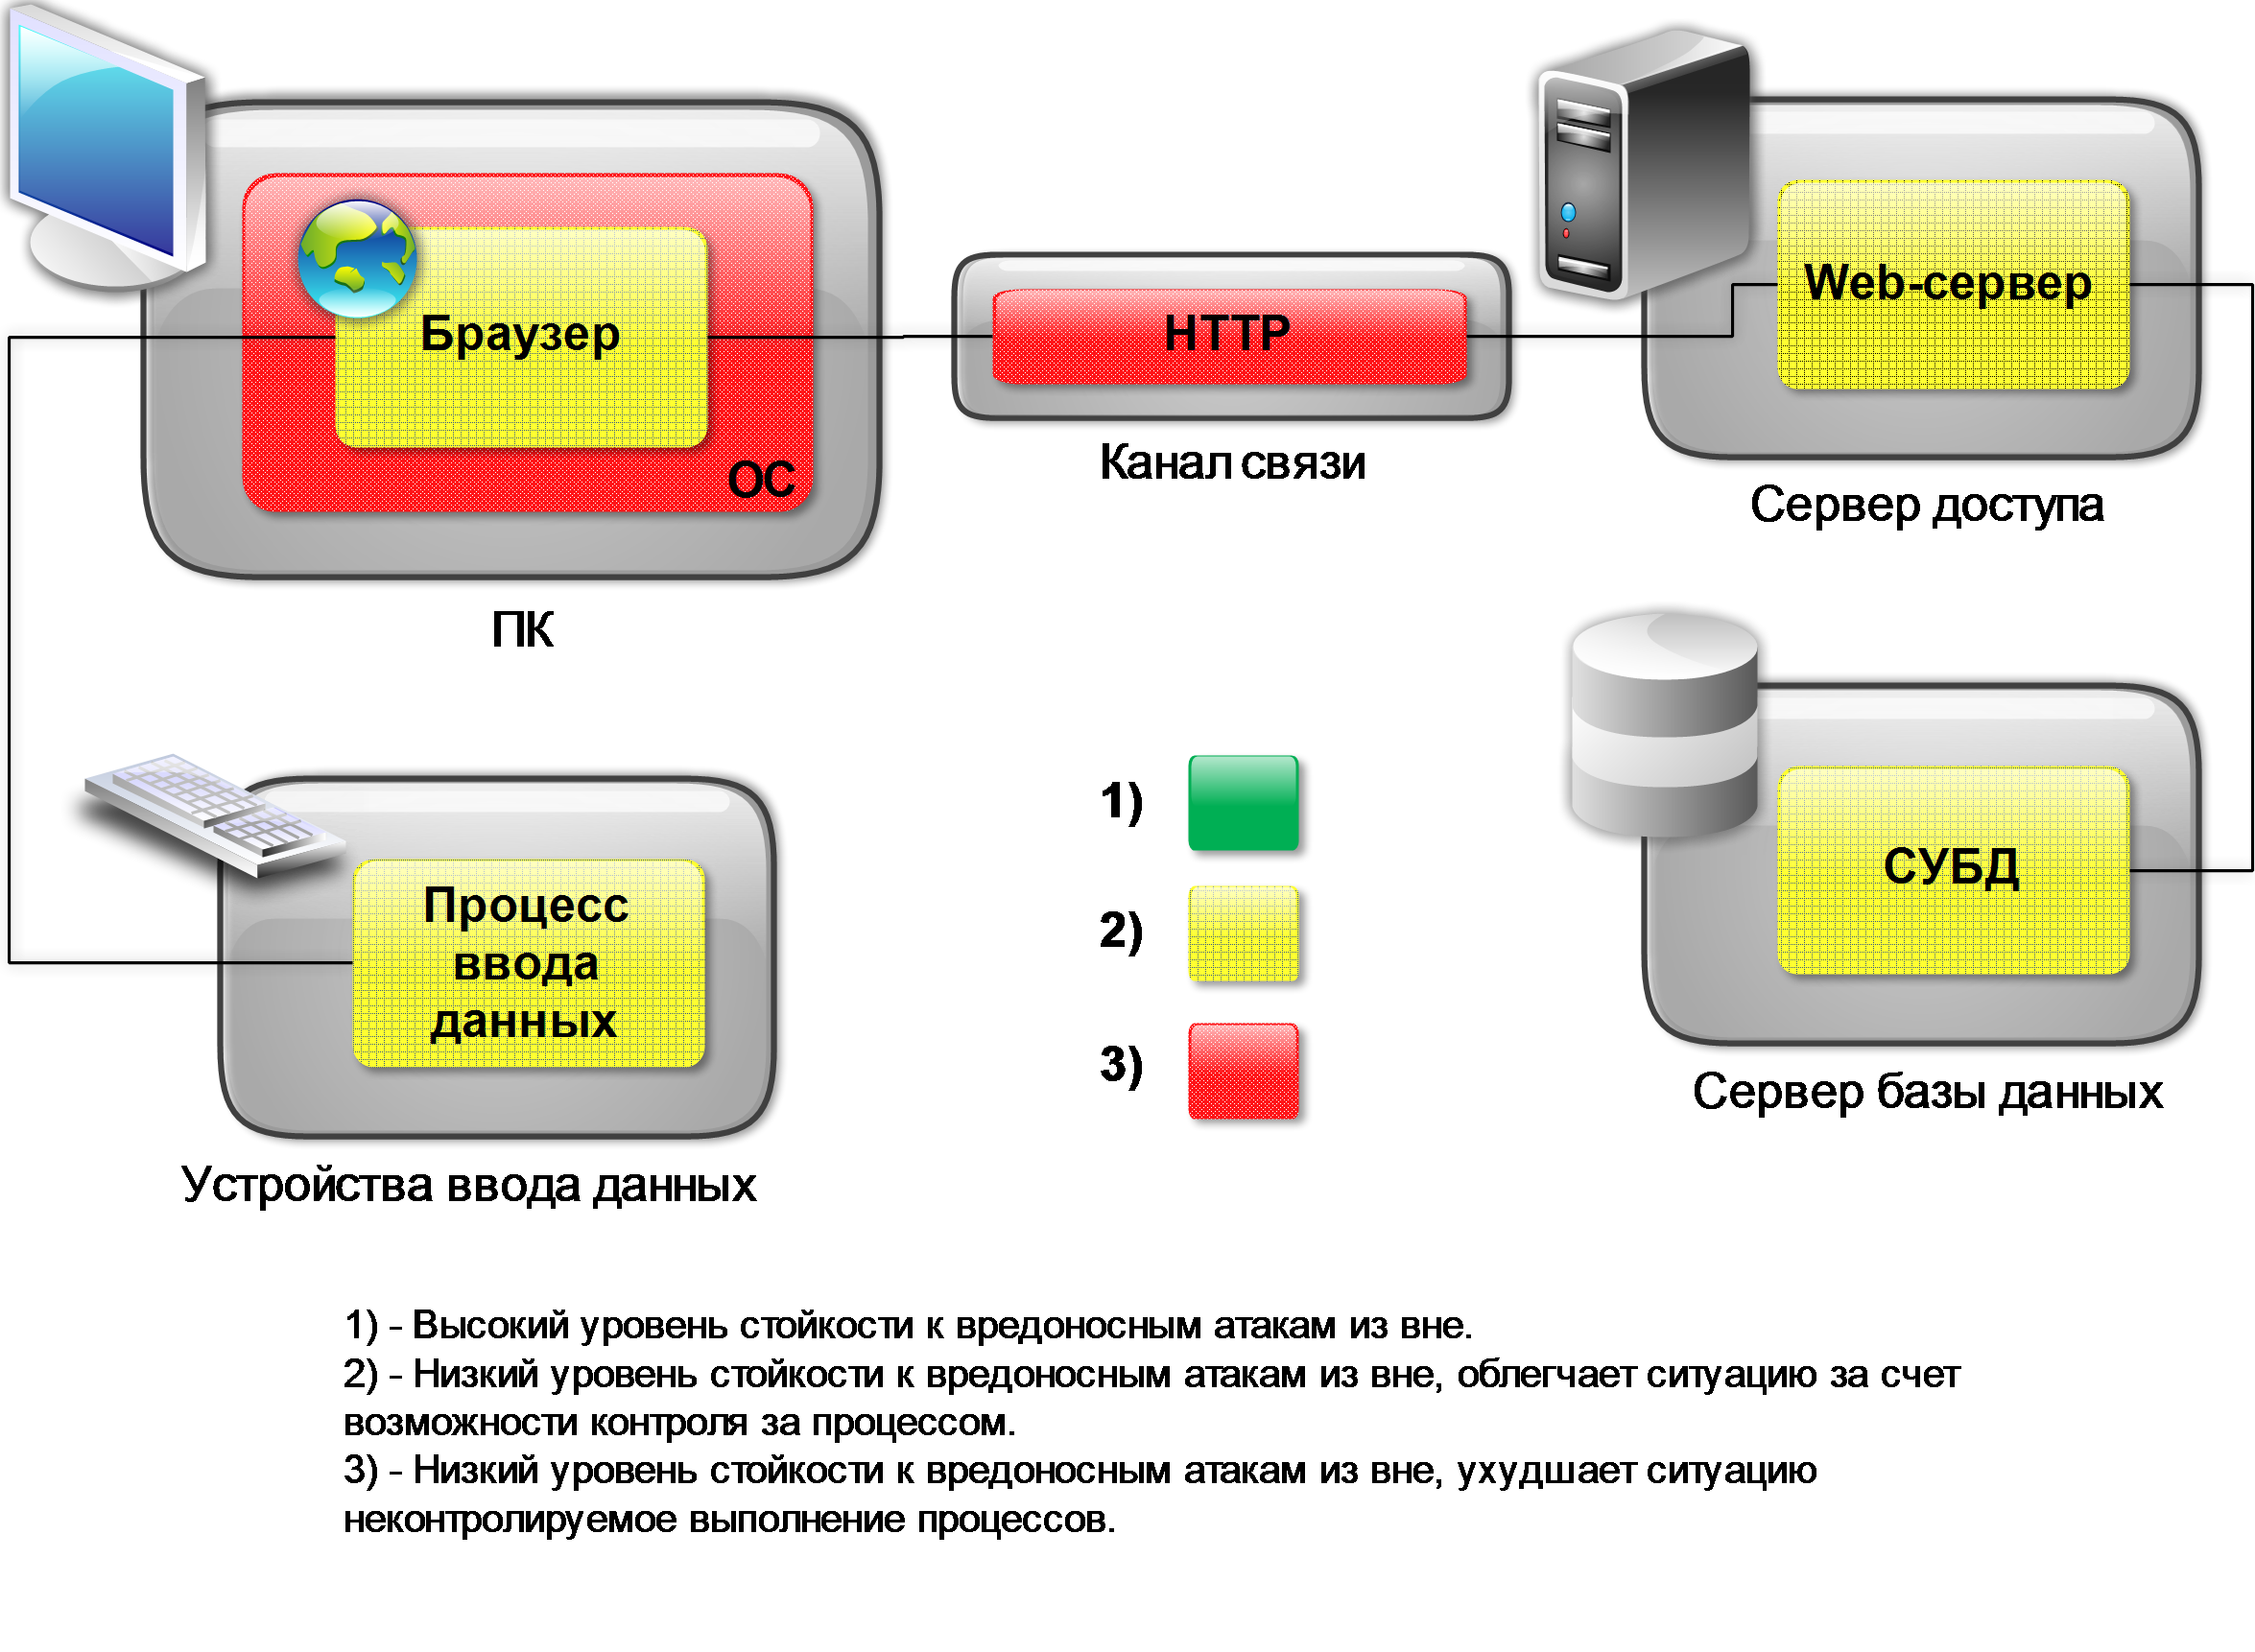
\includegraphics[width=1\linewidth]{2-1}}
\caption{Схема уязвимости узлов системы при традиционном подходе к
процессу аутентификации}
\label{ris:2.1}
\end{figure}

Детально рассмотрим уязвимости, которым подвержен каждый элемент системы в
отдельности.

\textit{Устройства ввода данных}, как правило, представляет собой клавиатуру. В
процессе аутентификации клавиатура может быть использована при вводе пароля. Данное
устройство включено в группу риска по следующим причинам:
\begin{itemize}
  \item данные (в частности пароль), вводимые с клавиатуры, могут быть
  доступными третьему лицу в результате банального слежения за процессом ввода;
  \item в результате целенаправленных действий злоумышленника клавиатура может
  быть сопряжена со специальным прослушивающим устройством, которое фиксирует
  все вводимые данные.
\end{itemize}

\textit{Персональный компьютер} входить в группу повышенной опасности из за
уязъвимостей операционных систем. В частности, угрозы могут исходить из
хаккерских атак, а так же от различных вредоносных программ, целенаправленно
собирающих секретную информацию. Ситуация осложняется из-за
неконтролируемого выполнения процессов, что не дает возможности определить
источник угрозы на ранних этапах.

\textit{Канал связи} является наиболее уязвимым местом любой системы, так как
информация передается абсолютно открытым образом, где практически каждый может
получить к ней доступ.

\textit{Серверная часть системы} так же включена в группу риска, не смотря на
высокие возможности обеспечения безопасности. Любая атака со стороны
злоумышленников может привести к полному отказу в работе системы и необратимым
последствиям.

Применение нового подхода к процессу аутентификации пользователей в сети с
использованием портативного цифрового ключа доступа снижает уровень уязвимости в
отдельных компонентах системы, особенно это касается критических участков. Это
можно проследить на рисунке~\ref{ris:2.2}).

 \begin{figure}[h]
\center{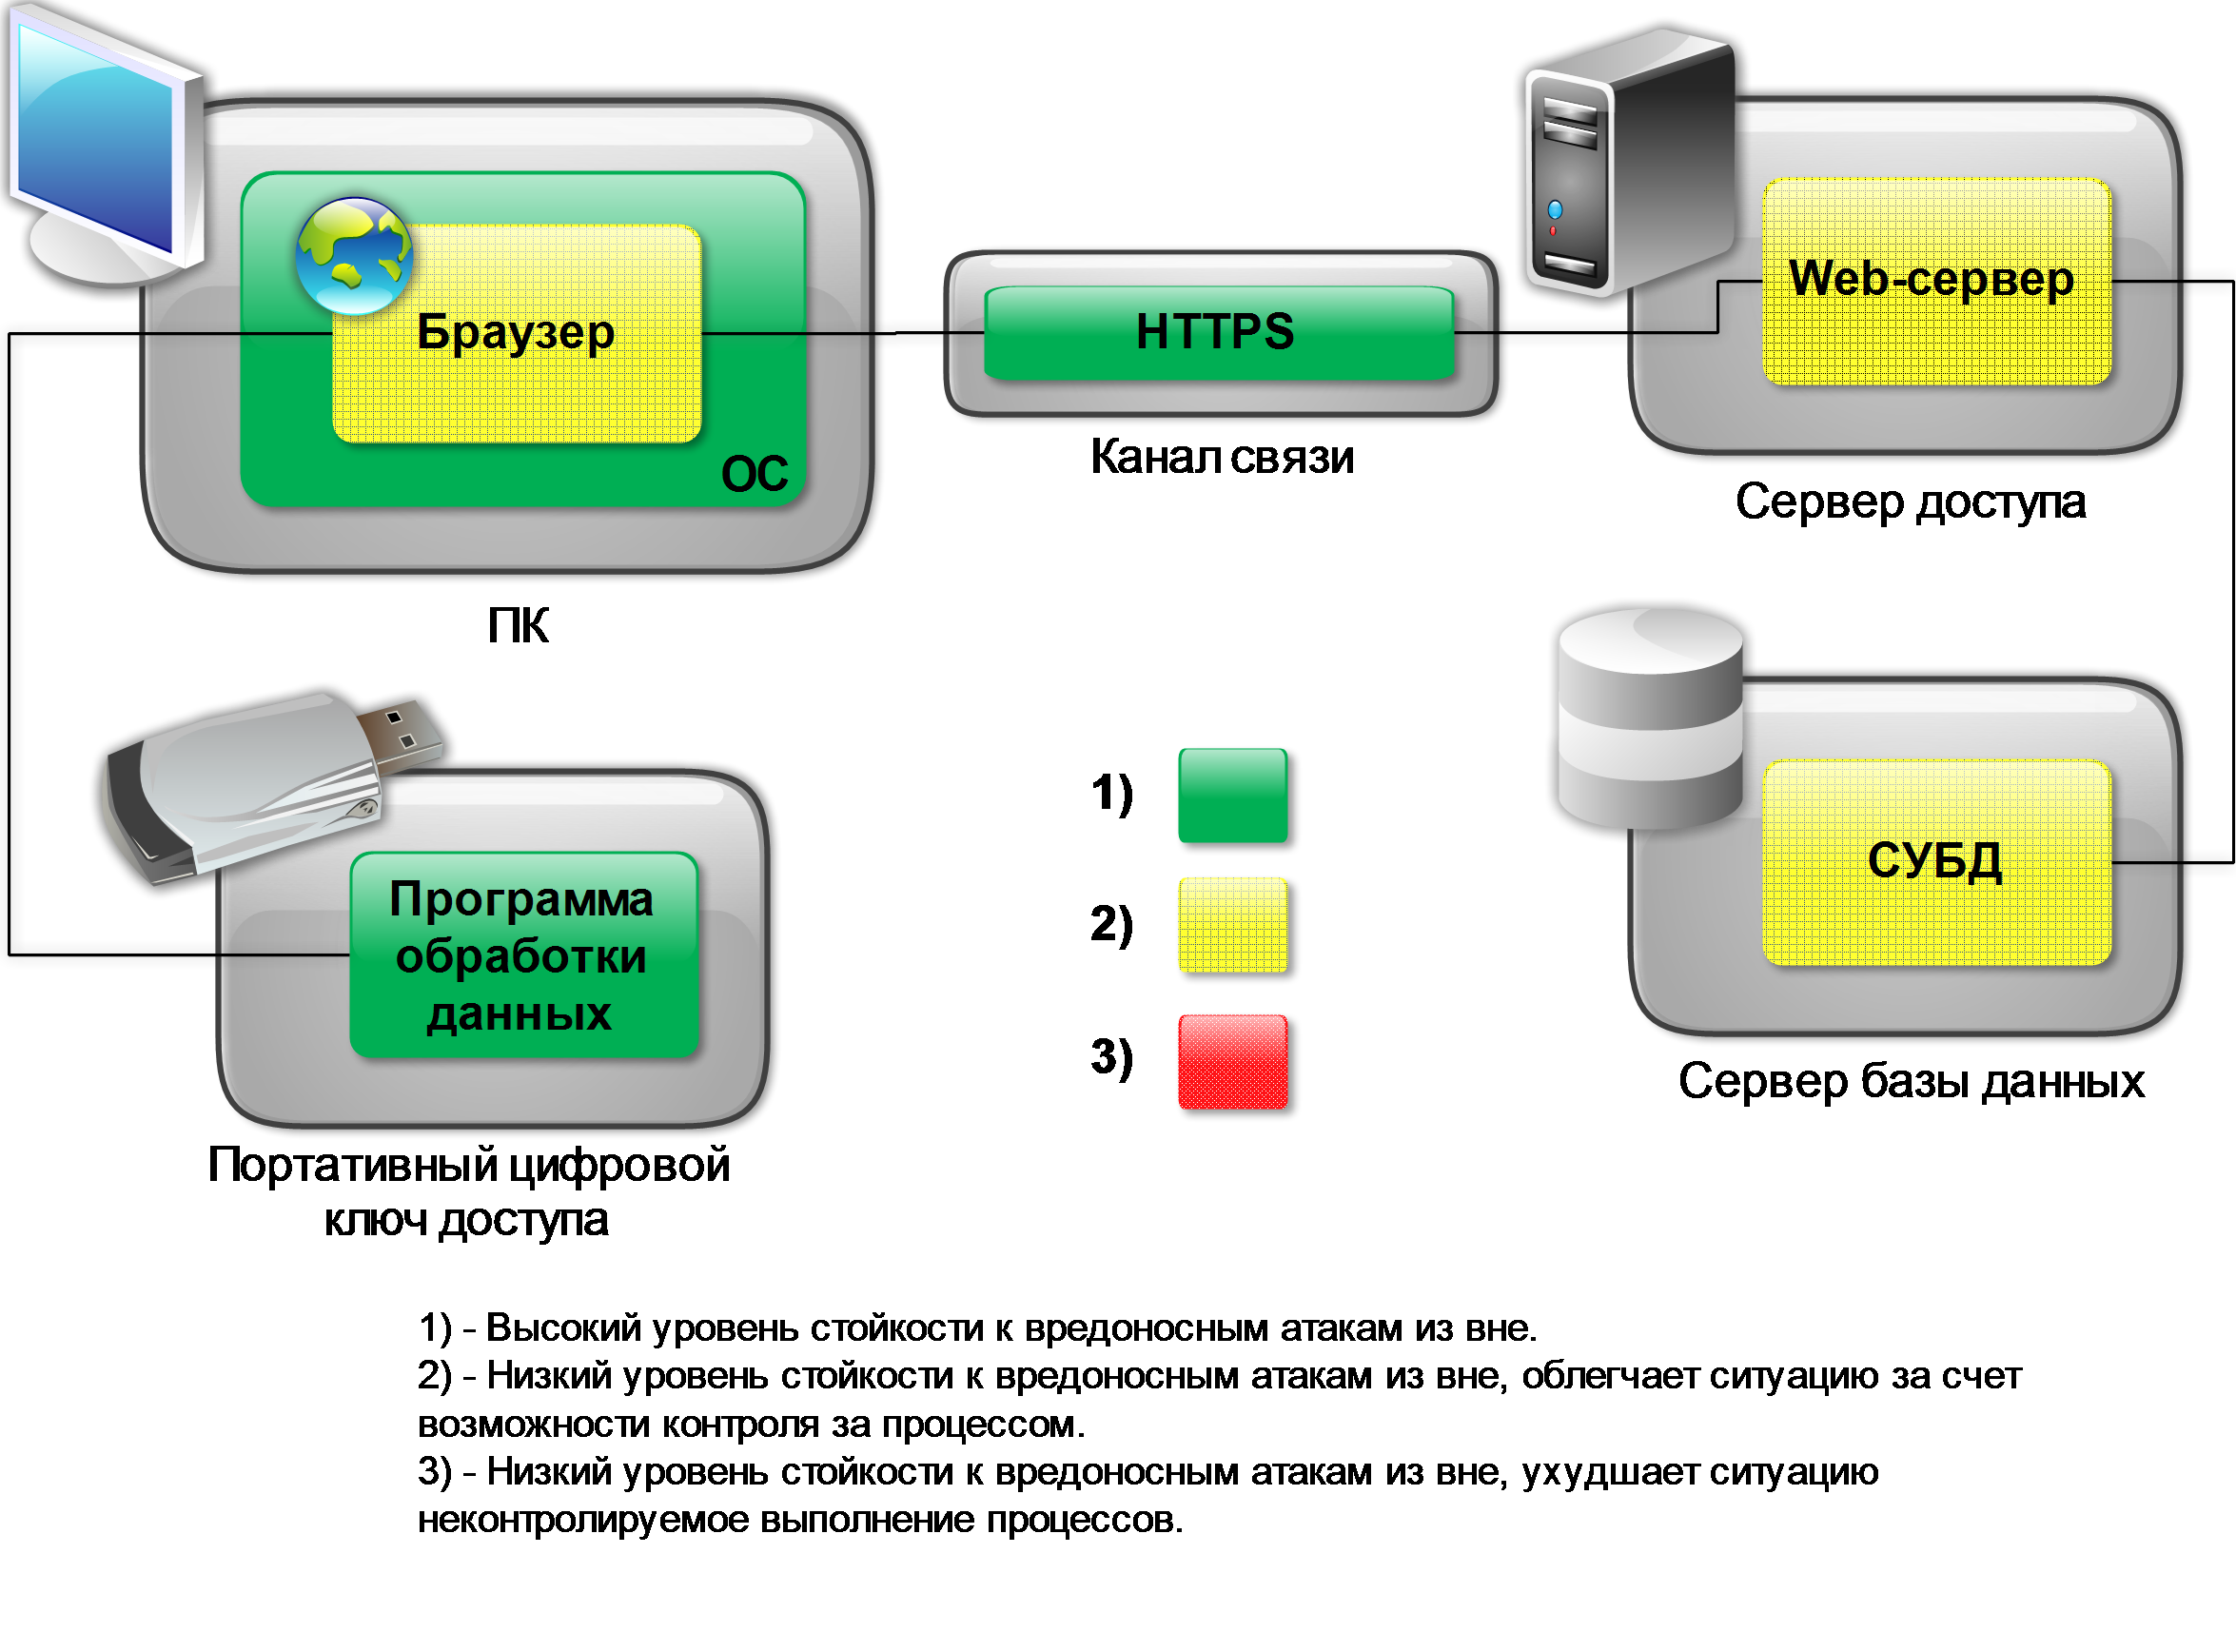
\includegraphics[width=1\linewidth]{2-2}}
\caption{Схема уязвимости узлов системы при новом подходе к процессу аутентификации}
\label{ris:2.2} 
\end{figure}


Выявленные улучшения достигаются с помощью:
\begin{itemize}
  \item Применяемых алгоритмов шифрования данных;
  \item Применения новой технологии хранения ключей и обработки алгоритмов
шифрования.
\end{itemize}

Применяемые алгоритмы шифрования обеспечивают безопасность передаваемых данных
при условии полной секретности ключей. 
  
Алгоритмы шифрования можно разделить на две категории:
\begin{itemize}
  \item алгоритмы симметричного шифрования;
  \item алгоритмы асимметричного шифрования.
\end{itemize}
	
В алгоритмах \textit{симметричного шифрования} для расшифрования обычно
используется тот же самый ключ, что и для зашифрования, или ключ, связанный с ним каким-либо
простым соотношением. Последнее встречается существенно реже, особенно в
современных алгоритмах шифрования. Такой ключ (общий для зашифрования и
расшифрования) обычно называется просто ключом шифрования.
Одним из наиболее распространенных алгоритмов данного вида является 
\textbf{DES} -- федеральный стандарт шифрования США в 1977-2001 годах,
разработанный группой под руководством доктора У. Тачмена. Архитектурой данного
алгоритма является классическая сбалансированная сеть Файстеля с начальной и
конечной битовыми перестановками общего вида. Длина ключа данного алгоритма
составляет 56 бит.

В \textit{асимметричном шифровании} ключ зашифрования $k_{1}$ легко вычисляется
из ключа $k_{2}$ таким образом, что обратное вычисление невозможно. Например, соотношение
ключей может быть таким:
\begin{equation}
k_{1} = a^{k_{2}} \ mod \ p ,
\end{equation}

где $a$ и $p$ -- параметры алгоритма шифрования, имеющие достаточно большую
размерность.

Яркими примерами данного вида шифрования являются алгоритмы \textbf{RSA} и
\textbf{ElGamal}.
Алгоритм RSA - Защищен патентом США N 4405829. Разработан в 1977 году в
Массачусетском технологическом институте (США). Получил название по первым
буквам фамилий авторов (Rivest, Shamir, Adleman). Криптостойкость основана на
вычислительной сложности задачи разложения большого числа на простые множители.
Алгоритм ElGamal разработан в 1985 году. Назван по фамилии автора - Эль-Гамаль.
Используется в стандарте США на цифровую подпись DSS (Digital Signature
Standard). Криптостойкость основана на вычислительной сложности задачи
логарифмирования целых чисел в конечных полях.~\cite{elgamal}

Еще одной разнавидностью асимметричных алгоритмов шифрования является
\textit{алгоритм электронно-цифровой подписи} (ЭЦП). Электронная подпись (ЭП) —
информация в электронной форме, которая присоединена к другой информации в электронной форме
(подписываемой информации) или иным образом связана с такой информацией и
которая используется для определения лица, подписывающего информацию.~\cite{FZ_63}
По своему существу электронная подпись представляет собой реквизит электронного
документа, позволяющий установить отсутствие искажения информации в электронном
документе с момента формирования ЭП и проверить принадлежность подписи владельцу
сертификата ключа ЭП. Значение реквизита получается в результате
криптографического преобразования информации с использованием закрытого ключа
ЭП.

Все существующие алгоритмы ЭЦП построены по единому принципу.
Разница заключается лишь в математической реализации отдельно взятого алгоритма.
Это связано с тем, что каждый новый алгоритм получает улучшения, по двум
основным направлениям:
повышение криптостойкости и снижение временных затрат и вычислительных ресурсов,
при этом схема генерации и верификации шифра остаётся неизменной.

Для уяснения сущности алгоритма рассмотрим математические принципы, на которых
они базируются. Все математические операции можно разделить на две части:
вычисление дайджеста подписываемого документа и сам алгоритм вычисления и
проверки шифра.
\begin{enumerate}
  \item Хеширование применяется для сравнения данных: если у двух массивов
  хеш-коды разные, массивы гарантированно различаются; если одинаковые --
  массивы, скорее всего, одинаковы. В общем случае однозначного соответствия
  между исходными данными и хеш-кодом нет в силу того, что количество значений
  хеш-функций меньше, чем вариантов входного массива; существует множество
  массивов, дающих одинаковые хеш-коды -- так называемые коллизии. Вероятность
  возникновения коллизий играет немаловажную роль в оценке качества хеш-функций.
Среди множества существующих хеш-функций принято выделять криптографически
стойкие, применяемые в криптографии. Для того, чтобы хеш-функция $H$ считалась
криптографически стойкой, она должна удовлетворять трем основным требованиям, на
которых основано большинство применений хеш-функций в криптографии:
	\begin{itemize}
	  \item Необратимость: для заданного значения хеш-функции m должно быть
	  вычислительно неосуществимо найти блок данных $X$, для которого $H(X) = m$;
	  \item Стойкость к коллизиям первого рода: для заданного сообщения $M$ должно
	  быть вычислительно неосуществимо подобрать другое сообщение $N$, для которого
	  $H(N) = H(M)$;
	  \item Стойкость к коллизиям второго рода: должно быть вычислительно
	  неосуществимо подобрать пару сообщений (М, М'), имеющих одинаковый хеш.
	\end{itemize}
	
Данные требования не являются независимыми:
  \begin{itemize}
    \item Обратимая функция нестойка к коллизиям первого и второго рода;
	\item Функция, нестойкая к коллизиям первого рода, нестойка к коллизиям второго
	рода; обратное неверно.
  \end{itemize}
	
Следует отметить, что не доказано существование необратимых хеш-функций, для
которых вычисление какого-либо прообраза заданного значения хеш-функции
теоретически невозможно. Обычно нахождение обратного значения является лишь
вычислительно сложной задачей.
Для криптографических хеш-функций также важно, чтобы при малейшем изменении
аргумента значение функции сильно изменялось (лавинный эффект). В частности,
значение хеша не должно давать утечки информации даже об отдельных битах
аргумента.~\cite{barichev}
  \item В источниках~\cite{GOST_P341094} и~\cite{ECP} описание алгоритма
  вычисления и проверки ЭЦП сформулированно следующим образом.
Пусть $x$ и $y$ это закрытый и открытый ключ соответственно. Такая пара является
единственной. Существует функция $y=p(x)$, которая связывает $x$ и $y$ и,
благодаря которой функции вычисления и проверки подписи становятся взаимообратными. Так же
существует группа параметров $Q$, которая является открытой, и не должна
меняться в пределах подписания и проверки одного документа. Пусть М -- текст
сообщения или документа, которые необходимо подписать с помощью электронной
подписи. Функция $h(M)$ вычисляет хеш сообщения. Пусть существует функция $t(x,
h(M), Q, k)$, где $k$ -- случайное число, генерируемое каждый раз, при
вычислении электронной подписи документа, тогда $r = t(x, h(M), Q, k)$ -- шифр,
существующая в открытом виде, доступная всем, а в первую очередь получателю.
Получателю известно само сообщение $M$, параметры алгоритма $Q$ и открытый ключ
отправителя $y$, а так же электронно-цифровая подпись к текущему документу,
которую сгенерировал отправитель,  назовём её $r'$, и, которая должна совпадать
с r, но возможно подверглась изменениям в результате действий злоумышленника.
Функция $v=t'(y, H(M), Q)$ вычисляет аналогичный шифр, но на данном этапе это
происходит уже с помощью открытого ключа. Таким образом, при равенстве $r'$ и
$v$ можно сделать вывод о том, что подпись и сам документ признается подлинным.
Существует важное ограничение, накладываемое на параметры $Q$. В силу того, что
в алгоритмах используются операция $mod$ (остаток от деления), не имеющая
обратной, тем самым обозначая логику защиты алгоритма, параметры $Q$ должны быть простые
числа. Кроме того, данные параметры должны быть «длинными» числами, причём, чем
«длиннее» число, тем выше криптостойкость алгоритма. Ключи алгоритма $x$ и $y$
берутся на основе параметров $Q$.
  \end{enumerate}

\textit{Новая технология} подразумевает использование специализированного
аппаратного средства для хранения ключей и обработки алгоритмов шифрования.
Данное устройство позволяет организовать безопасное хранение секретных ключей.
Программное средство, функционирующее на данном устройстве, предоставляет очень
узкий интерфейс обмена данными и малый набор команд, поэтому считать секретный
ключ с устройства не представляется возможным. Кроме того, для обеспечения
защиты ключа от несанкционированного копирования или кражи,  все алгоритмы
шифрования выполняются на данном устройстве. Таким образом, секретные ключи
имеют высочайшую степень защиты, что делает их абсолютно неуязвимыми на всех
этапах прохождения процедуры аутентификации пользователя в сети.

Кроме этого, помимо осуществления аутентификации пользователя в сети
корпоративных порталов, новая методика имеет широкие возможности для создания
инструментов проверки подлинности документов, поскольку данные процессы
практически идентичны с точки зрения реализации.
 